\section{Probabilistic Notation}
\begin{frame}{Probabilistic Notation}
    \textbf{Sequence Notation Basics}

    Sentence: $w_1, w_2, \ldots, w_n$

    For example: $w_1 = \text{I},\ w_2 = \text{love},\ w_3 = \text{NLP}$

    \vspace{1em}
    \textbf{General representation:}
    \begin{itemize}
        \item Unigram: $P(w_i)$
        \item Bigram: $P(w_i \mid w_{i-1})$
        \item Trigram: $P(w_i \mid w_{i-2},\ w_{i-1})$
    \end{itemize}
\end{frame}

\begin{frame}{Unigram probability}
    \begin{figure}
        \centering
        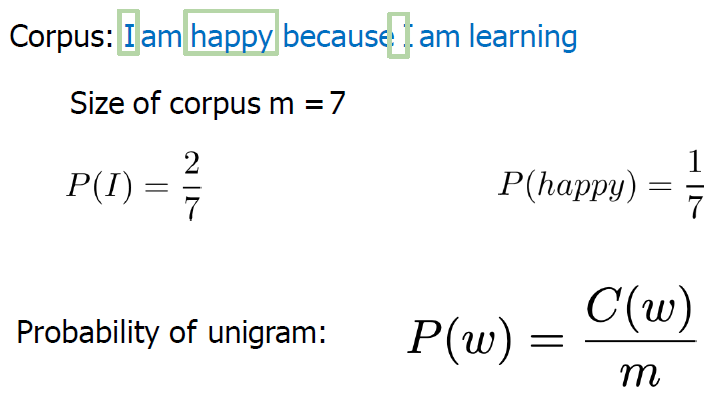
\includegraphics[width=\textwidth,height=0.8\textheight,keepaspectratio]{images/nlp-intro/unigram-probability.png}
    \end{figure}
\end{frame}

\begin{frame}{Bigram probability}
    \begin{figure}
        \centering
        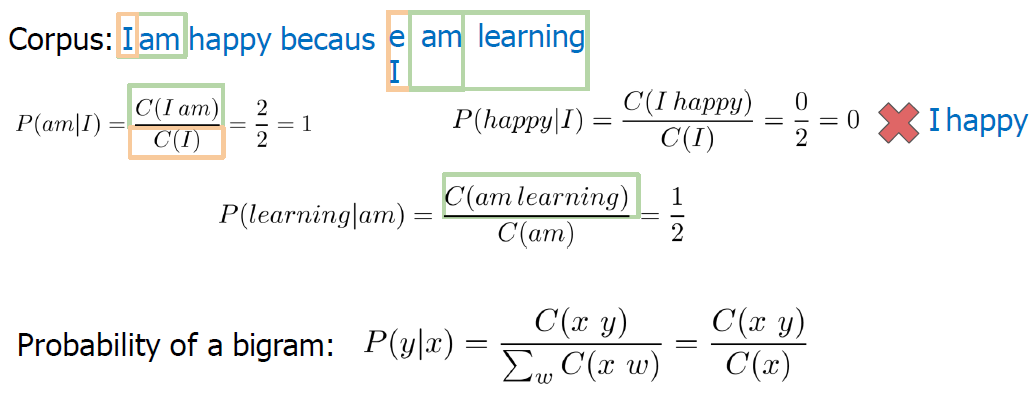
\includegraphics[width=\textwidth,height=0.8\textheight,keepaspectratio]{images/nlp-intro/bigram-probability.png}
    \end{figure}
\end{frame}

\begin{frame}{Trigram probability}
    \begin{figure}
        \centering
        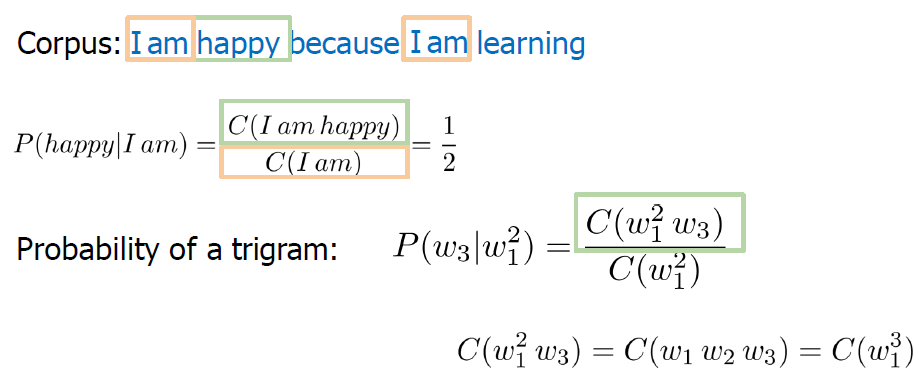
\includegraphics[width=\textwidth,height=0.8\textheight,keepaspectratio]{images/nlp-intro/trigram-probability.png}
    \end{figure}
\end{frame}

\begin{frame}{N-gram probability}
    \begin{figure}
        \centering
        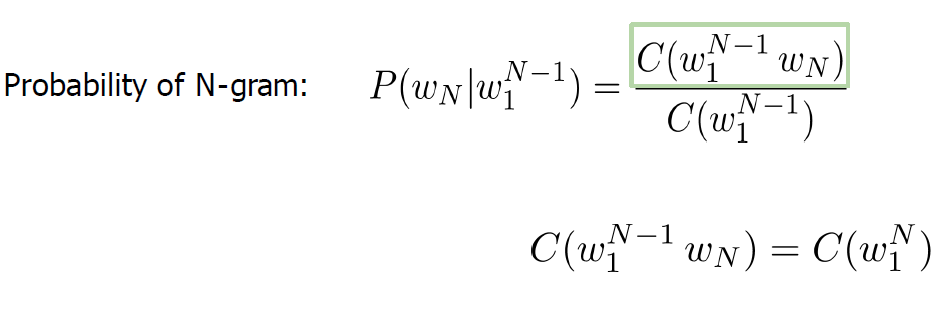
\includegraphics[width=\textwidth,height=0.8\textheight,keepaspectratio]{images/nlp-intro/ngram-probability.png}
    \end{figure}
\end{frame}

\begin{frame}{N-gram Language Modeling}
    \textbf{Objective:} Compute the probability of a sentence

    \vspace{1em}
    \textbf{N-gram Assumption:} The probability of a word depends only on the previous $(n-1)$ words.

    \vspace{1em}
    \textbf{Formula:}
    \[
        P(w_1^n) \approx \prod_{i=1}^{n} P(w_i \mid w_{i-n+1}^{i-1})
    \]
    where $w_1^n$ denotes the sequence $w_1, w_2, \ldots, w_n$ and $w_{i-n+1}^{i-1}$ is the context of the previous $(n-1)$ words.
\end{frame}

\begin{frame}{Estimating Probabilities: Maximum Likelihood Estimation (MLE)}
    \textbf{Bigram MLE:}

    \[
        P(w_i \mid w_{i-1}) = \frac{\text{Count}(w_{i-1}, w_i)}{\text{Count}(w_{i-1})}
    \]

    \begin{itemize}
        \item $\text{Count}(w_{i-1}, w_i)$: Number of times the bigram $(w_{i-1}, w_i)$ appears in the corpus.
        \item $\text{Count}(w_{i-1})$: Number of times the word $w_{i-1}$ appears as a context.
    \end{itemize}
\end{frame}

\begin{frame}{Example: Bigram Probabilities}
    \textbf{Text:} ``I love NLP. I love AI.''

    \vspace{1em}
    \textbf{Bigrams and Counts:}
    \begin{itemize}
        \item (I, love): 2
        \item (love, NLP): 1
        \item (love, AI): 1
    \end{itemize}

    \vspace{1em}
    \textbf{Probability Calculations:}
    \begin{itemize}
        \item $P(\text{love} \mid \text{I}) = \frac{2}{2} = 1.0$
        \item $P(\text{NLP} \mid \text{love}) = \frac{1}{2} = 0.5$
        \item $P(\text{AI} \mid \text{love}) = \frac{1}{2} = 0.5$
    \end{itemize}
\end{frame}